% Set up the document
\documentclass{article}

% Page size
\usepackage[
    letterpaper,]{geometry}

% Lines between paragraphs
\setlength{\parskip}{\baselineskip}
\setlength{\parindent}{0pt}

% Math
\usepackage{mathtools}
\usepackage{amssymb}
\usepackage{amsthm}
\usepackage{commath}

% Number sets
\newcommand{\C}{\mathcal{C}}
\newcommand{\N}{\mathbb{N}}
\newcommand{\Q}{\mathbb{Q}}
\newcommand{\R}{\mathbb{R}}
\newcommand{\Z}{\mathbb{Z}}

% Links
\usepackage{hyperref}

% Page numbers at top right
\usepackage{fancyhdr}
\pagestyle{fancy}
\fancyhf{}
\fancyhead[R]{\thepage}
\renewcommand\headrulewidth{0pt}

% Graphics
\usepackage{float}
\usepackage{graphicx}
\graphicspath{ {./img/} }

\begin{document}

\textbf{MATH 461 assignment 1} \\
\textbf{Matt Wiens \#301294492} \\
\textbf{2020-05-22}

1.4.1. Assume you have a culture of bacteria crowing in a petri dish,
and each cell divides into two identical copies of itself every 10
minutes.

(a) Choose a unit time, and find the corresponding probability of cell division.

\textit{Solution.}

Let the unit of time be $\Delta t = 1 \text{ minute}$. Then the
corresponding probability of cell division during any given minute is
given by
%
\begin{equation*}
    \frac{1}{10 \Delta t} \cdot \Delta t = 10\%
    .
\end{equation*}

\newpage

(b) Write down a discrete-time model which balances the amount of cells
at time $t$ and at time $t + \Delta t$.

\textit{Solution.}

Let $N(t)$ denote the number of cells existing at time $t$. Then we have
the discrete time-time model
%
\begin{equation*}
    N(t + \Delta t) = N(t) + 0.1 (2 N(t)) = 1.2 N(t)
    .
\end{equation*}
%
The second term $0.1 (2 N(t))$ in the second part of the equation
reflects that there is a 10\% chance that any individual cell in the
population will split into two cells.

\newpage

(c) Define the growth rate, and derive the corresponding continuous-time model.

\textit{Solution.}

Rearranging the equation in part b and dividing through by $\Delta t$ we obtain
%
\begin{equation*}
    \frac{N(t + \Delta t) - N(t)}{\Delta t} = \frac{0.2}{\Delta t} N(t)
    .
\end{equation*}
%
We can immediately identify the growth rate as 2 cells per minute. We can
also read off the corresponding continuous-time model
%
\begin{equation*}
    \dod{}{t} N(t) = 0.2 N(t)
\end{equation*}
%
where the units on both sides of the equation are number of cells per minute.

\newpage

(d) Solve both the discrete-time model and continuous-time models, and
compare the solutions.

\textit{Solution.}

We'll first the discrete-time model
%
\begin{equation*}
    N(t + \Delta t) = 1.2 N(t)
    .
\end{equation*}
%
Here we'll define $N_i \coloneqq N(i \cdot \Delta t)$ and so we can rewrite
our model as
%
\begin{equation*}
    N_{i + 1} = 1.2 N_i
    .
\end{equation*}
%
If at time 0 (the initial time) we have $N_0$ cells then we can write
the solution as
%
\begin{equation*}
    N_i = (1.2)^i N_0
    .
\end{equation*}
%
For the continuous-time model
%
\begin{equation*}
    \dod{}{t} N(t) = 0.2 N(t)
\end{equation*}
%
we can read off the solution
%
\begin{equation*}
    N(t) = e^{0.2 t}
    .
\end{equation*}

\newpage

(e) When is a discrete-time model appropriate? When is a continuous-time
model appropriate?

\textit{Solution.}

If we are dealing with inherently discrete quantities that stay small in
number (for example, the number of mice in a house) then a continuous
model might give results that aren't useful (e.g., that hypothetically
there might be 1.5 mice in a house). In other circumstances, when either
dealing with continuous quantities or discrete quantities that are
expected to grow large in number, a continuous model is likely more
appropriate.

\newpage

1.4.2. Study the two models (1.2), (1.1) which lead to Figure 1.2 (all
  numbered references are referring to the course textbook) and vary the
  time increment $\Delta t$ (e.g., try $\Delta t = \frac{1}{4} \text{
  day}$, $\frac{1}{8} \text{ day}$, $1 \text{ day}$, $2 \text{ days}$,
  $10 \text{ days}$). What do you observe? Which choice of $\Delta t$
  gives the best, and which gives the worst agreement? Can you explain
  why?

\textit{Solution.}

In Figure~\ref{fig:142} below we see the effect of using different time
steps with the disease model presented in the textbook. We see that the
smaller the time step, the better the agreement with the continuous
model. This should be expected, because we obtained the continuous model
by taking $\Delta t \to 0$ in the discrete model; so the smaller our time
step, the closer we get to the continuous model.
%
\begin{figure}[ht]
    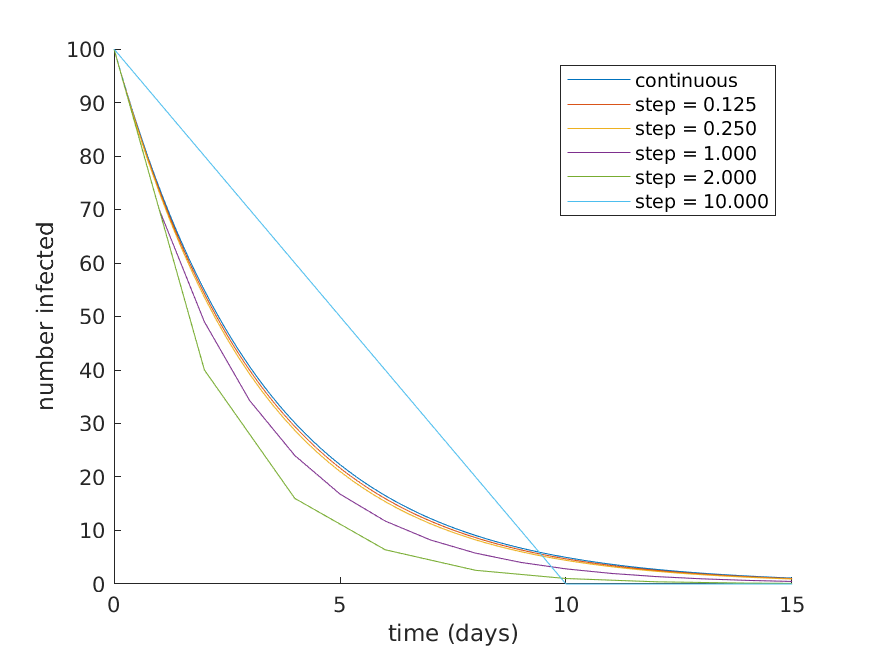
\includegraphics[width=35em]{q142}
    \centering
    \caption{Effect of different time steps on disease model ($\alpha = 0.3$)}
    \label{fig:142}
\end{figure}

\end{document}
